\begin{frame}{Ils ont quelles qualités?}
  \begin{columns}
    \column{0.5\textwidth}
      \begin{center}
        Têtes-à-claques \\
        \href{https://youtu.be/l1s5zyQbo2c?si=_zbGkN0o1zQ9aO-S}{
          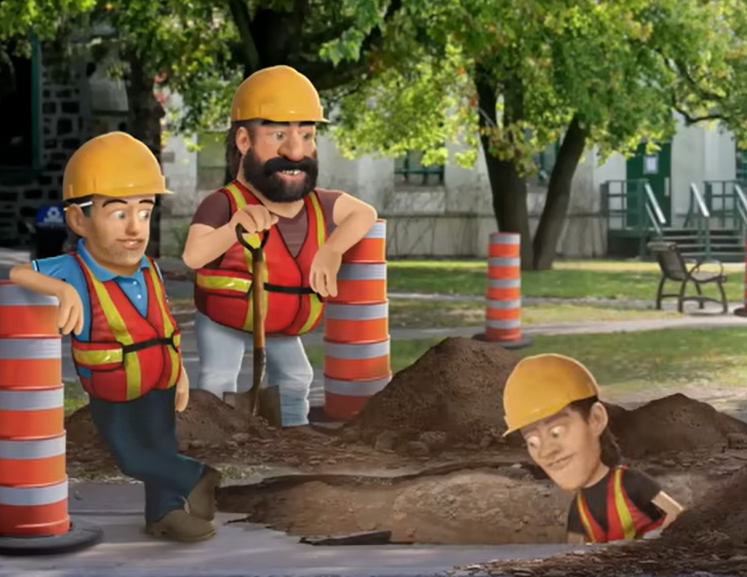
\includegraphics[scale=0.3]{slaquer.png}
        } \\
        Ces ouvriers, comment sont-ils?
      \end{center}
    \column{0.5\textwidth}
      \uncover<2>{
        En groupes, discutez de ce que font les membres de chaque classe sociale aux États-Unis au-dessous.
        Posez des questions au groupe avec le vocabulaire aux pages 146 et 147.
        Par exemple:
        \begin{itemize}
          \item[] \textbf{Modèle:}
          \item \emph{Qui va à l'opéra?}
        \end{itemize}
        \begin{enumerate}
          \item la classe ouvrière
          \item la classe moyenne
          \item la bourgeoisie
          \item la grande bourgeoisie
        \end{enumerate}
      }
  \end{columns}
\end{frame}